%  !TeX  root  =  user_guide.tex

\chapter{Premiers Pas}\label{label_getstarted}

% when the revision of a section has been finalized, 
% comment out the following line:
% \updatedisclaimer

Ce chapitre donne un bref aperçu de l'installation de \qg, de quelques jeux de données provenant du site Internet et du lancement d'une première session d'affichage de couches matricielles et vectorielles.

\section{Installation}\label{label_installation}
\index{installation}

L'installation de \qg est très simple. Des installateurs sont disponibles pour les systèmes d'exploitation \mswin et \mac. Beaucoup de distributions \tux mettent à disposition des fichiers binaires précompilés (.rpm ou .deb) ou des dépôts sources via leurs interfaces de gestion de logiciels. Vous pouvez obtenir les dernières informations concernant les paquets binaires sur le site de \qg sur \url{download.qgis.org}.

\minisec{Installation à partir des sources}

Si vous désirez installer \qg à  partir des sources, veuillez vous référer au guide de programmation et de compilation disponible sur \url{http://www.qgis.org/en/documentation/manuals.html}.
Les instructions d'installation sont également diffusées avec le code source de \qg.

\minisec{Installation sur un support amovible}

\qg vous permet de définir une option --configpath qui remplace le chemin par défaut (~/.qgis) pour la configuration utilisateur et oblige QSettings à l'utiliser. Cela permet à l'utilisateur de transporter son installation de \qg sur une clé USB avec ses extensions et paramètres.

\section{Échantillon de données}\label{label_sampledata}
\index{Échantillon de données}

Le guide de l'utilisateur contient des exemples basés sur le jeu de données échantillon inclus dans \qg.

\win L'installateur \mswin possède une option qui permet de télécharger le jeu de données échantillon \qg.
Si vous le cochez, les données seront téléchargées dans votre répertoire intitulé \filename{Mes Documents} et placées dans le répertoire \filename{GIS Database}. Vous pouvez utiliser l'explorateur \mswin pour vous déplacer à partir de ce répertoire vers un autre répertoire de votre choix.
Si vous ne cochez pas cette option durant l'installation, vous pouvez :
\begin{itemize}[label=--]
\item utiliser les données que vous possédez déjà,
\item télécharger l'échantillon sur le site de \qg
 \url{http://download.qgis.org} ou
\item désinstaller et réinstaller \qg en cochant, cette fois, la case de téléchargement.
\end{itemize}

\bigskip

\nix \osx Pour les systèmes \tux et \mac il n'y a pas encore de paquets disponibles sous forme de rpm, deb ou dmg. Pour utiliser 
l'échantillon de données, téléchargez le fichier compressé \filename{qgis\_sample\_data} au format ZIP ou archive TAR depuis 
\url{http://download.osgeo.org/qgis/data/}
et décompressez-le à l'endroit de votre choix. Le jeu de données sur l'Alaska comporte toutes les données SIG qui ont servi à la préparation des captures d'écran et des exemples qui figurent dans ce manuel. La projection est l'Alaska Albers Equal Area qui a pour unité le pied et dont le code EPSG est le 2964.

\begin{verbatim}
PROJCS["Albers Equal Area",
    GEOGCS["NAD27",
        DATUM["North_American_Datum_1927",
            SPHEROID["Clarke 1866",6378206.4,294.978698213898,
                AUTHORITY["EPSG","7008"]],
            TOWGS84[-3,142,183,0,0,0,0],
            AUTHORITY["EPSG","6267"]],
        PRIMEM["Greenwich",0,
            AUTHORITY["EPSG","8901"]],
        UNIT["degree",0.0174532925199433,
            AUTHORITY["EPSG","9108"]],
        AUTHORITY["EPSG","4267"]],
    PROJECTION["Albers_Conic_Equal_Area"],
    PARAMETER["standard_parallel_1",55],
    PARAMETER["standard_parallel_2",65],
    PARAMETER["latitude_of_center",50],
    PARAMETER["longitude_of_center",-154],
    PARAMETER["false_easting",0],
    PARAMETER["false_northing",0],
    UNIT["us_survey_feet",0.3048006096012192]]
\end{verbatim}

Si vous désirez utiliser \qg comme une interface à \grass, vous trouverez une sélection d'échantillons de secteurs (e.g. Spearfish ou South Dakota) sur le site officiel de \grass \\
\url{http://grass.osgeo.org/download/data.php}. 

\section{Étape pratique}\label{samplesession}

Maintenant que vous avez \qg d'installé avec un échantillon de données disponible, nous aimerions vous faire une courte démonstration. Vous allez visualiser une couche raster et une couche vectorielle.

Nous allons utiliser la couche raster landcover \filename{qgis\_sample\_data/raster/landcover.img} 
et la couche vectorielle des lacs \filename{qgis\_sample\_data/gml/lakes.gml}.

\minisec{Démarrer \qg}

\begin{itemize}[label=--]
\item \nix{Démarrer \qg en tapant: \usertext{qgis} en ligne de commande dans une console ou, 
si vous utilisez un fichier binaire précompilé, depuis le menu Application.}
\item \win{Démarrer \qg en utilisant le menu Démarrer, un raccourci placé sur le Bureau, 
ou double-cliquez sur un fichier de projet existant de \qg.}
\item \osx{Double-cliquez sur l'icône de \qg dans votre répertoire du menu Applications.}
\end{itemize} 

\begin{figure}[ht]
   \begin{center} 
   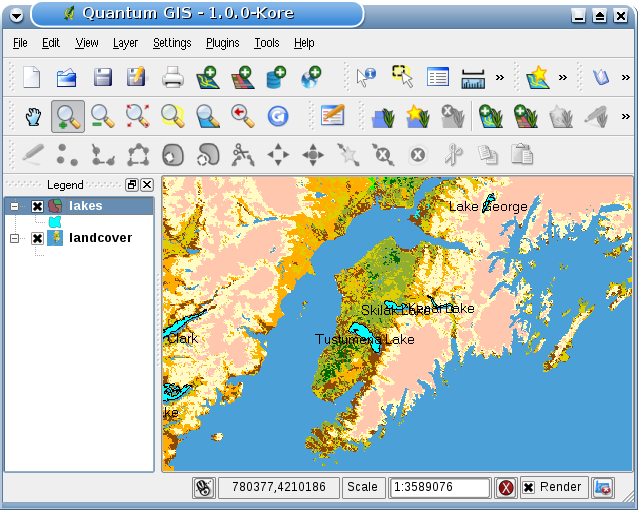
\includegraphics[clip=true, width=12cm]{simple_session}
   \caption{Une session de \qg  \nixcaption}\label{fig:simple_session}
\end{center}
\end{figure}

\minisec{Charger les couches raster et vecteur depuis le jeu de données}
{\setlength{\baselineskip}{1.3\baselineskip}
\begin{enumerate}[itemsep=2pt]
\item Cliquez sur l'icône \toolbtntwo{mActionAddRasterLayer}{Ajouter une couche Raster}.
\item Parcourez le dossier \filename{qgis\_sample\_data/raster/}, sélectionnez 
le fichier ERDAS img\\
 \filename{landcover.img} et cliquez \button{Ouvrir}.
\item Si le fichier n'est pas listé, vérifiez le type de fichier à partir du menu déroulant 
au dessous de la boîte de dialogue afin de filtrer le bon type de fichier, dans ce cas-ci c'est \selectstring{Fichiers de type}{Erdas Imagine (*.img, *.IMG)}
\item Maintenant cliquez sur l'icône \toolbtntwo{mActionAddOgrLayer}{Ajouter une couche vecteur}. 
\item \radiobuttonon{Fichier} devrait être sélectionné comme Type de source dans la nouvelle boîte de dialogue 
\dialog{Ajouter une couche vecteur}. Maintenant cliquez \button{Parcourir} pour sélectionner la couche vecteur
\item Parcourez le répertoire \filename{qgis\_sample\_data/gml/}, sélectionnez "GML"
à partir du menu déroulant Type de fichier, sélectionnez le fichier GML \filename{lakes.gml}, cliquez sur \button{Ouvrir}, et enfin, dans la boîte de dialogue Ajouter une couche vecteur, cliquez \button{OK}.
\item Zoomez sur une zone de votre choix avec quelques lacs.
\item Double-cliquez la couche \filename{lakes} dans la liste des cartes pour ouvrir la fenêtre\\ \dialog{Propriétés de la couche}.
\item Cliquez sur l'onglet \tab{Style} et sélectionnez le bleu comme couleur de remplissage.
\item Cliquez sur l'onglet \tab{Étiquettes} et cochez la case \checkbox{Afficher les étiquettes} pour permettre l'étiquetage des entités. 
Choisissez le champ intitulé NAMES comme champ d'étiquetage.
\item Pour améliorer la lisibilité des étiquettes, vous pouvez ajouter un halo autour d'eux,
en cliquant sur ``tampon'' dans la liste à gauche puis \checkbox{Étiquettes tampon}. Choisissez 3 comme taille du tampon.
\item Cliquez \button{Appliquez} pour vérifier si le résultat est satisfaisant et enfin cliquez sur \button{OK}.
\end{enumerate} 

Vous pouvez constater combien il est facile d'afficher des couches raster ou vecteur dans \qg. Passons aux sections suivantes pour en apprendre plus sur les autres fonctionnalités, caractéristiques et paramètres disponibles et sur la façon de les utiliser.

\FloatBarrier
